%%%%%%%%%%%%%%%%%%%% book.tex %%%%%%%%%%%%%%%%%%%%%%%%%%%%%
%
% sample root file for the chapters of your "monograph"
%
% Use this file as a template for your own input.
%
%%%%%%%%%%%%%%%% Springer-Verlag %%%%%%%%%%%%%%%%%%%%%%%%%%


% RECOMMENDED %%%%%%%%%%%%%%%%%%%%%%%%%%%%%%%%%%%%%%%%%%%%%%%%%%%
\documentclass[pdftex,12pt, oneside]{book}
 
% choose options for [] as required from the list
% in the Reference Guide, Sect. 2.2
%\usepackage[paperwidth=8.5in, paperheight=13in]{geometry} %Folio
\usepackage[paperwidth=8.27in, paperheight=11.69in]{geometry} %A4

\usepackage{makeidx}         % allows index generation
\usepackage{graphicx}        % standard LaTeX graphics tool
                             % when including figure files
\usepackage[bottom]{footmisc}% places footnotes at page bottom
\usepackage[bahasa]{babel}
\usepackage{enumerate}
\usepackage{paralist}
\usepackage{float}
\usepackage{gensymb}  
\usepackage{listings}
\usepackage{color}
\renewcommand{\baselinestretch}{1.5}

\newcommand{\HRule}{\rule{\linewidth}{0.5mm}}

\makeindex             % used for the subject index
                       % please use the style svind.ist with
                       % your makeindex 
                     
\definecolor{codegreen}{rgb}{0,0.6,0}
\definecolor{codegray}{rgb}{0.5,0.5,0.5}
\definecolor{codepurple}{rgb}{0.58,0,0.82}
\definecolor{backcolor}{rgb}{0.95,0.95,0.92}

\lstdefinestyle{mystyle}{
  backgroundcolor=\color{backcolor},
  commentstyle=\color{codegreen},
  keywordstyle=\color{magenta},
  stringstyle=\color{codepurple},
  basicstyle=\footnotesize,
  breakatwhitespace=false,
  breaklines=true,
  captionpos=b,
  keepspaces=true,
  numbers=left,
  numbersep=5pt,
  showspaces=false,
  showstringspaces=false,
  showtabs=false,
  tabsize=2
}

\lstset{style=mystyle}


%%%%%%%%%%%%%%%%%%%%%%%%%%%%%%%%%%%%%%%%%%%%%%%%%%%%%%%%%%%%%%%%%%%%%

\begin{document}
\sloppy


\begin{titlepage}

\begin{center}
{\large DOKUMENTASI RANCANGAN SISTEM BASIS DATA UNTUK SISTEM INFORMASI PEMBAYARAN PAJAK BUMI DAN BANGUNAN PERDESAAN DAN PERKOTAAN DI KABUPATEN BREBES}

\HRule\\[1cm]

PERIODE PENILAIAN TAHUN 2018\\[1cm]


\includegraphics[width=0.5\textwidth]{./resources/logo}\\[1cm]

Oleh :\\
Priyanto Tamami, S.Kom.\\
NIP 19840409 201001 1 025\\


\vfill


Fungsional Pranata Komputer\\
Badan Pengelolaan Pendapatan, Keuangan dan Aset Daerah\\
Pemerintah Daerah Kabupaten Brebes\\
Brebes, 19 Maret 2018
\end{center}

\end{titlepage}

\frontmatter%%%%%%%%%%%%%%%%%%%%%%%%%%%%%%%%%%%%%%%%%%%%%%%%%%%%%%


\begin{center}
{\huge \bfseries Lembar Pengesahan}\\[0.4cm]

\begin{tabular}{l c p{10cm}}
  Nama Kegiatan & : & 	Membuat Petunjuk Operasional Sistem Komputer \\
  Judul & : & PETUNJUK PENGOPERASIAN PROGRAM SISTEM INFORMASI PEMBAYARAN PAJAK BUMI DAN BANGUNAN PERDESAAN DAN PERKOTAAN DI KABUPATEN BREBES \\
\end{tabular}\\[2cm]

\begin{tabular}{c c}
  Disetujui oleh : & Disusun Oleh \\
  Kepala Sub Bidang Keberatan & Pranata Komputer \\
  Pada tanggal 18 April 2018 & Selesai tanggal : 17 April 2018 \\
  & \\
  & \\
  & \\
  M.L. Setiyawan, S.E.Ak & Priyanto Tamami, S.Kom \\
  NIP 19790530 200604 1 006 & NIP 19840409 201001 1 025
\end{tabular}

\end{center}  

\tableofcontents
\listoffigures

\mainmatter%%%%%%%%%%%%%%%%%%%%%%%%%%%%%%%%%%%%%%%%%%%%%%%%%%%%%%%
\chapter{TAHAPAN IMPLEMENTASI}

Tahapan dari implementasi sistem basis data untuk sistem informasi pembayaran Pajak Bumi dan Bangunan Perdesaan dan Perkotaan (PBB-P2) meliputi kegiatan-kegiatan seperti berikut ini :

\section{Persiapan Perangkat Keras}

Persiapan yang dilakukan terhadap perangkat keras tentunya menyediakan ruang untuk sistem basis data dipasangkan, baik perangkat keras peladen, besarnya memori yang diperlukan, serta ruang simpanan pada media \textit{harddisk}.

Karena sistem informasi yang dibangun masih menggunakan sistem basis data milik SISMIOP (Sistem Manajemen Informasi Objek Pajak) untuk Pajak Bumi dan Bangunan Perdesaan dan Perkotaan (PBB-P2), artinya perangkat keras untuk implementasi telah siap dan dapat digunakan.

\section{Persiapan Perangkat Lunak}

Persiapan perangkat lunak yang diperlukan dalam hal ini adalah sistem operasi dan sistem basis data yang akan digunakan.

Karena sistem basis data yang diakses oleh sistem informasi ini menggunakan satu basis data yang sama dengan SISMIOP (Sistem Manajemen Informasi Objek Pajak) untuk Pajak Bumi dan Bangunan Perdesaan dan Perkotaan (PBB-P2), maka perangkat lunaknya telah siap terpasang dan siap untuk digunakan.

Perangkat lunak yang digunakan sebagai sistem operasi adalah Windows Server 2008 R2, sedangkan sistem basis data menggunakan Oracle 11g.

\section{Persiapan Basis Data}

Sistem basis data yang digunakan akan berjenis \textit{Relational Database Management System} (RDBMS), dengan menggunakan Oracle 11g.

Sistem informasi yang dibangun akan menggunakan pencatatan pembayaran dari SISMIOP (Sistem Manajemen Informasi Objek Pajak) milik Pajak Bumi dan Bangunan Perdesaan dan Perkotaan (PBB-P2), sehingga struktur basis datanya telah terbentuk hanya tinggal melakukan akses saja ke beberapa tabel yang berhubungan dengan pencatatan pembayaran Pajak Bumi dan Bangunan Perdesaan dan Perkotaan (PBB-P2).

\section{Persiapan Fasilitas Fisik}

Persiapan fisik pun telah dilakukan diantaranya kesiapan jaringan sehingga peladen aplikasi dapat dan mampu melakukan akses ke peladen sistem basis data.

Kondisi jaringan dipastikan stabil menggunakan kabel UTP (\textit{Unshielded Twisted Pair}), karena nantinya peladen aplikasi akan selalu melakukan akses ke peladen sistem basis data setiap ada permintaan atau \textit{request} dari klien.

\section{Pelatihan Pemakai}

Tidak ada pemakai atau pengguna yang berhubungan langsung dengan sistem basis data, sehingga tidak diperlukan pelatihan bagi pengguna. Nantinya pengguna atau pemakai akan melakukan akses ke peladen aplikasi untuk mendapatkan informasi yang diinginkan, kemudian peladen aplikasi yang akan melakukan pengambilan data ke peladen basis data apabila datanya tersedia.
%04.rancangan
\chapter{RANCANGAN BASIS DATA}

Rancangan struktur basis data akan terdiri dari beberapa tabel seperti berikut :

\section{Tabel SPPT}

Tabel ini selain mencatatkan ketetapan untuk tiap objek pajak pada tiap tahun pajak, tabel ini juga mencatatkan status pembayaran apakah sudah lunas atau belum pada kolom / \textit{field} \texttt{status\_pembayaran\_sppt}. Struktur tabelnya adalah seperti pada gambar \ref{fig:tab-sppt} berikut ini :

\begin{figure}[H]
	\centering
	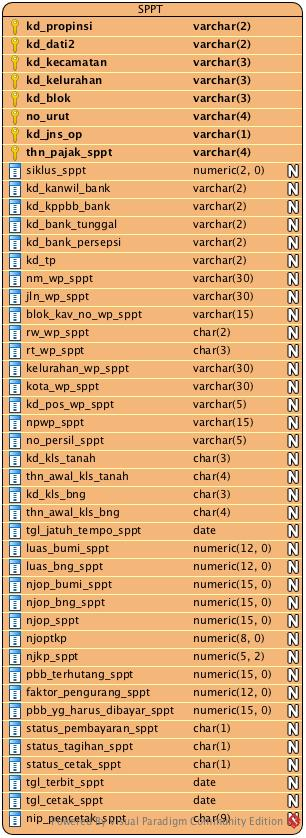
\includegraphics[width=0.5\textwidth]{./resources/struktur-tabel-sppt}
	\caption{Struktur Tabel SPPT}
	\label{fig:tab-sppt}
\end{figure}

Kolom atau \textit{field} yang dimanfaatkan dari tabel ini hanya beberapa bagian saja, yaitu :

\begin{itemize}
	\item Nomor Objek Pajak (NOP), yang terdiri dari \textit{field} atau kolom \texttt{kd\_propinsi}, \texttt{kd\_dati2}, \texttt{kd\_kecamatan}, \texttt{kd\_kelurahan}, \texttt{kd\_blok}, \texttt{no\_urut}, dan \texttt{kd\_jns\_op}.
	\item Tahun pajak pada \textit{field} atau kolom \texttt{thn\_pajak\_sppt}.
	\item Nama wajib pajak pada \textit{field} atau kolom \texttt{nm\_wp\_sppt}
	\item Besarnya pajak terhutang pada \textit{field} atau kolom \texttt{pbb\_yg\_harus\_dibayar\_sppt}
	\item Status pembayaran pada \textit{field} atau kolom \texttt{status\_pembayaran\_sppt}
\end{itemize}

\section{Tabel DAT\_OBJEK\_PAJAK}

Tabel \texttt{DAT\_OBJEK\_PAJAK}, digunakan untuk menampilkan informasi mengenai objek pajak seperti alamat, luas bumi dan bangunan, serta Nilai Jual Objek Bumi dan Bangunan. Struktur tabel dari \texttt{DAT\_OBJEK\_PAJAK} adalah seperti pada gambar \ref{fig:tab-dat-op} berikut ini :

\begin{figure}[H]	
	\centering
	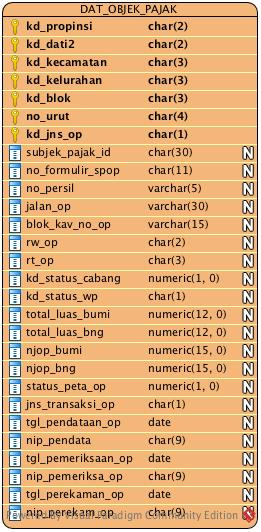
\includegraphics[width=0.3\textwidth]{./resources/struktur-tabel-dat-op}
	\caption{Struktur Tabel \texttt{DAT\_OBJEK\_PAJAK}}
	\label{fig:tab-dat-op}
\end{figure}

\section{Tabel DAT\_SUBJEK\_PAJAK}

Tabel \texttt{DAT\_SUBJEK\_PAJAK} ini digunakan untuk menampilkan informasi mengenai subjek pajaknya seperti nama dan alamatnya. Struktur tabel dari \texttt{DAT\_SUBJEK\_PAJAK} ini adalah seperti pada gambar \ref{fig:tab-dat-sp} berikut ini :

\begin{figure}[H]
	\centering
	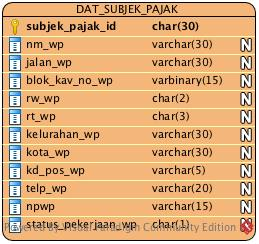
\includegraphics[width=0.3\textwidth]{./resources/struktur-tabel-dat-sp}
	\caption{Struktur Tabel \texttt{DAT\_SUBJEK\_PAJAK}}
	\label{fig:tab-dat-sp}
\end{figure}

\section{Tabel REF\_KECAMATAN}

Untuk tabel \texttt{REF\_KECAMATAN} digunakan hanya untuk menampilkan informasi nama Kecamatan dimana objek berada. Struktur tabel untuk \texttt{REF\_KECAMATAN} ini seperti terlihat pada gambar \ref{fig:tab-ref-kec} berikut ini :

\begin{figure}[H]
	\centering
	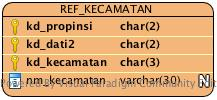
\includegraphics[width=0.3\textwidth]{./resources/struktur-tabel-ref-kec}
	\caption{Struktur Tabel \texttt{REF\_KECAMATAN}}
	\label{fig:tab-ref-kec}
\end{figure}

\section{Tabel REF\_KELURAHAN}

Tabel \texttt{REF\_KELURAHAN} pun digunakan hanya untuk menampilkan nama Kelurahan / Desa dimana objek pajak berada. Struktur tabel \texttt{REF\_KELURAHAN} ini seperti terlihat pada gambar \ref{fig:tab-ref-kel} berikut ini :

\begin{figure}[H]
	\centering
	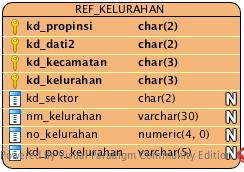
\includegraphics[width=0.3\textwidth]{./resources/struktur-tabel-ref-kel}
	\caption{Struktur Tabel \texttt{REF\_KELURAHAN}}
	\label{fig:tab-ref-kel}
\end{figure}


\chapter{LOKASI SISTEM BASIS DATA}

Karena sistem yang dibangun akan menampilkan informasi pencatatan pembayaran dari Pajak Bumi dan Bangunan sektor Perdesaan dan Perkotaan (PBB-P2), maka lokasi dari sistem basis data ini masih bergabung atau menjadi satu dengan sistem basis data milik Sistem Manajemen Informasi Objek Pajak (SISMIOP) yang digunakan untuk mengelola Pajak Bumi dan Bangunan Perdesaan dan Perkotaan (PBB-P2).

Sistem Manajemen Informasi Objek Pajak (SISMIOP) ini aplikasi lengkap berbasis \textit{desktop} yang mampu melakukan manajemen atau pengelolaan data dari awal pendataan sampai pelaporan realisasi pembayarannya, sehingga apabila ingin menampilkan informasi pencatatan pembayaran yang lengkap akan lebih baik untuk melakukan akses langsung terhadap sistem basis datanya.
\chapter{SKEMA DAN KAMUS DATA}

\section{Skema Basis Data}

Skema relasi dari sistem basis data yang akan digunakan pada sistem informasi pencatatan pembayaran ini seperti terlihat pada gambar \ref{fig:dia-relasi-entity} berikut ini :

\begin{figure}[H]
	\centering
	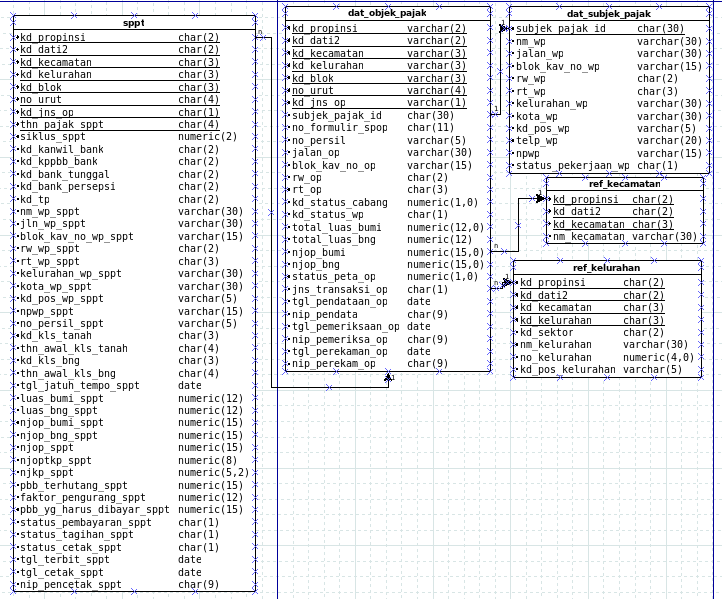
\includegraphics[width=1\textwidth]{./resources/db-diagram}
	\caption{Skema Relasi \textit{Entity}}
	\label{fig:dia-relasi-entity}
\end{figure}

Akses utama aplikasi ini ada pada tabel \texttt{SPPT}, dimana nantinya tiap data pada tabel ini akan memiliki relasi n:1 dengan tabel \texttt{DAT\_OBJEK\_PAJAK}, ini karena tiap objek pajak yang tercatat akan memiliki banyak data SPPT untuk tiap tahun pajak.

Setiap data pada tabel \texttt{DAT\_OBJEK\_PAJAK} akan memiliki relasi 1:1 dengan data pada tabel \texttt{DAT\_SUBJEK\_PAJAK}.

Sedangkan hubungan atau relasi antara tabel \texttt{DAT\_OBJEK\_PAJAK} dengan \texttt{REF\_KECAMATAN} dan \texttt{DAT\_OBJEK\_PAJAK} dengan \texttt{REF\_KELURAHAN} adalah n:1, dimana tiap 1 (satu) data pada tabel \texttt{REF\_KECAMATAN} atau \texttt{REF\_KELURAHAN} akan memiliki banyak objek pada tabel \texttt{DAT\_OBJEK\_PAJAK}.

\section{Kamus Data}

Pengertian dan isi data dari tiap tabel dan \textit{field} akan terbagi menjadi seperti berikut :

\subsection{Tabel SPPT}

Tabel ini akan menyimpan ketetapan untuk tiap objek pajak pada tiap tahun pajak, tabel ini pun menyimpan tanda status pembayaran yang apabila terisi dengan 1 (satu), maka tandanya telah terbayar. Penjelasan untuk masing-masing \textit{field} adalah sebagai berikut :

\begin{itemize}
	\item \texttt{kd\_propinsi} : Kode Propinsi yang berisi \texttt{33} (tiga tiga) yang artinya masuk dalam wilayah Propinsi Jawa Tengah.
	\item \texttt{kd\_dati2} : Kode Kabupaten/Kota yang berisi \texttt{29} (dua sembilan) yang artinya masuk dalam wilayah Kabupaten Brebes.
	\item \texttt{kd\_kecamatan} : Kode Kecamatan yang menjadi tanda atau pembeda masing-masing Kecamatan dalam wilayah Kabupaten Brebes. Daftarnya akan merujuk pada tabel \texttt{REF\_KECAMATAN}.
	\item \texttt{kd\_kelurahan} : Kode Kelurahan atau kode untuk Desa, yang menjadi tanda atau pembeda masing-masing Desa/Kelurahan dalam suatu wilayah Kecamatan. Rincian datanya akan merujuk ke tabel \texttt{REF\_KELURAHAN}.
	\item \texttt{kd\_blok} : Kode Blok yang menjadi tanda pemisah antar blok dalam satu wilayah Desa/Kelurahan.
	\item \texttt{no\_urut} : Nomor Urut yang menjadi penanda tiap objek pajak dalam satu wilayah blok.
	\item \texttt{kd\_jns\_op} : Kode Jenis Objek Pajak, yang menjadi tanda bahwa objek tersebut masuk dalam wilayah Perdesaan dan Perkotaan, atau dalam wilayah Perkebunan, Perhutanan, atau Pertambangan, dapat juga menjadi penanda bagi objek pajak bersama dan objek pajak induk.
	\item \texttt{thn\_pajak\_sppt} : Tahun Pajak SPPT (Surat Pemberitahuan Pajak Terhutang), yang menjadi tanda ketetapan untuk tahun pajak keberapa \textit{record} yang sedang diakses.
	\item \texttt{siklus\_sppt} : Siklus SPPT (Surat Pemberitahuan Pajak Terhutang), yang menjadi tanda sudah berapa kali objek pajak tersebut mengalami penetapan atau perubahan ketetapan.	
	\item \texttt{kd\_kanwil\_bank} : Kode Kantor Wilayah tempat Bank Kas Negara, ini bawaan struktur Dirjen Pajak Kementerian Keuangan dahulu.
	\item \texttt{kd\_kppbb\_bank} : Kode Kantor Pelayanan Pajak Bumi dan Bangunan (KP-PBB) tempat Bank Kas Negara, ini juga bawaan struktur Dirjen Pajak Kementerian Keuangan dahulu.,
	\item \texttt{kd\_bank\_tunggal} : Kode untuk Bank Kas Negara, ini struktur bawaan Dirjen Pajak Kementerian Keuangan sebelum Pajak Bumi dan Bangunan sektor Perdesaan dan Perkotaan dilimpahkan ke Daerah.
	\item \texttt{kd\_bank\_persepsi} : Kode untuk Bank Persepsi yang juga merupakan struktur pengelolaan Pajak Bumi dan Bangunan sektor Perdesaan dan Perkotaan yang masih ditangani Dirjen Pajak Kementerian Keuangan.
	\item \texttt{kd\_tp} : Kode Tempat Pembayaran untuk Pajak Bumi dan Bangunan sektor Perdesaan dan Perkotaan.
	\item \texttt{nm\_wp\_sppt} : Nama wajib pajak yang ditetapkan pada Surat Pemberitahuan Pajak Terhutang (SPPT).
	\item \texttt{jln\_wp\_sppt} : nama jalan dari alamat tempat tinggal wajib pajak.
	\item \texttt{blok\_kav\_no\_wp\_sppt} : nomor blok, kavling, atau nomor rumah atau tempat tinggal wajib pajak
	\item \texttt{rw\_wp\_sppt} : nomor RW alamat tempat tinggal wajib pajak.
	\item \texttt{rt\_wp\_sppt} : nomor RT alamat tempat tinggal wajib pajak
	\item \texttt{kelurahan\_wp\_sppt} : nama kelurahan dari alamat tempat tinggal wajib pajak
	\item \texttt{kota\_wp\_sppt} : nama Kota / Kabupaten dari alamat tempat tinggal wajib pajak
	\item \texttt{kd\_pos\_wp\_sppt} : kode pos dari alamat tempat tinggal wajib pajak.
	\item \texttt{npwp\_sppt} : Nomor NPWP dari wajib pajak
	\item \texttt{no\_persil\_sppt} : Nomor persil dari lokasi objek pajak
	\item \texttt{kd\_kls\_tanah} : Kode kelas tanah dari objek pajak yang akan menjadi referensi untuk melakukan akses data ke nilai tanah untuk tahun pajak tertentu.
	\item \texttt{thn\_awal\_kls\_tanah} : Tahun awal dari kode kelas tanah
	\item \texttt{kd\_kls\_bng} : Kode kelas bangunan dari objek yang akan menjadi referensi untuk melakukan penetapan nilai jual bangunan berdasarkan tahun pajak tertentu
	\item \texttt{thn\_awal\_kls\_bng} : Tahun awal dari kode kelas bangunan.
	\item \texttt{tgl\_jatuh\_tempo\_sppt} : Tanggal jatuh tempo untuk Surat Pemberitahuan Pajak Terhutang (SPPT) tersebut.
	\item \texttt{luas\_bumi\_sppt} : Luas bumi yang akan ditetapkan pada Surat Pemberitahuan Pajak Terhutang (SPPT).
	\item \texttt{luas\_bng\_sppt} : Luas bangunan yang akan ditetapkan pada Surat Pemberitahuan Pajak Terhutang (SPPT).
	\item \texttt{njop\_bumi\_sppt} : Nilai Jual Objek Pajak (NJOP) untuk nilai bumi keseluruhan.
	\item \texttt{njop\_bng\_sppt} : Nilai Jual Objek Pajak (NJOP) untuk nilai bangunan secara keseluruhan
	\item \texttt{njop\_sppt} : Nilai Jual Objek Pajak (NJOP) secara keseluruhan
	\item \texttt{njoptkp} : Nilai Jual Objek Pajak Tidak Kena Pajak (NJOPTKP) untuk objek yang bersangkutan yang ditetapkan tiap tahun.
	\item \texttt{njkp\_sppt} : Nilai Jual Kena Pajak (NJKP) untuk objek pajak yang didapat dari nilai NJOP secara keseluruhan dikurangi NJOPTKP.
	\item \texttt{pbb\_terhutang\_sppt} : Nilai Pajak Bumi dan Bangunan yang terhutang untuk tahun pajak tersebut.
	\item \texttt{faktor\_pengurang\_sppt} : Nilai yang menjadi pengurang pajak terhutang untuk tahun pajak tersebut apabila ada.
	\item \texttt{pbb\_yg\_harus\_dibayar\_sppt} : Besarnya Pajak Bumi dan Bangunan yang harus dibayarkan yang didapat dari nilai pajak terhutang dikurangi faktor pengurang.
	\item \texttt{status\_pembayaran\_sppt} : Status apakah pajak yang harus dibayarkan sudah terbayar atau belum, bila belum terbayar akan bernilai \texttt{0} (nol), apabila sudah terbayar akan bernilai \texttt{1} (satu), apabila ketetapan SPPT dibatalkan akan bernilai \texttt{2} (dua).
	\item \texttt{status\_tagihan\_sppt} : Status apakah SPPT tersebut sudah ditagihkan atau belum.
	\item \texttt{status\_cetak\_sppt} : Status pencetakan SPPT, apakah sudah tercetak yang bernilai \texttt{1} (satu), atau belum tercetak yang bernilai \texttt{0} (nol).
	\item \texttt{tgl\_terbit\_sppt} : Tanggal terbitnya SPPT
	\item \texttt{tgl\_cetak\_sppt} : Tanggal tercetaknya SPPT
	\item \texttt{nip\_pencetak\_sppt} : Kode pengguna yang melakukan pencetakan SPPT.
\end{itemize}

\subsection{Tabel DAT\_OBJEK\_PAJAK}

Tabel ini adalah tabel utama untuk menyimpan hasil perekaman data-data mengenai objek pajak. Penjelasan untuk masing-masing \textit{field} adalah sebagai berikut :

\begin{itemize}
	\item \texttt{kd\_propinsi} : Kode Propinsi yang bernilai \texttt{33} yang artinya propinsi Jawa Tengah.
	\item \texttt{kd\_dati2} : Kode Kabupaten/Kota yang bernilai \texttt{29} yang artinya Kabupaten Brebes.
	\item \texttt{kd\_kecamatan} : Kode Kecamatan yang terdiri dari 3 (tiga) digit sebagai tanda pembeda antar Kecamatan dalam wilayah Kabupaten.
	\item \texttt{kd\_kelurahan} : Kode Kelurahan / Desa yang terdiri dari 3 (tiga) digit sebagai tanda pembeda antar Desa / Kelurahan dalam suatu wilayah Kecamatan.
	\item \texttt{kd\_blok} : Kode blok yang terdiri dari 3 (tiga) digit sebagai tanda pembeda antar blok dalam satu wilayah Desa / Kelurahan.
	\item \texttt{no\_urut} : Nomor urut dari tiap objek pajak dalam sebuah wilayah blok.
	\item \texttt{kd\_jns\_op} : Kode Jenis Objek Pajak, sebagai pembeda apakah ini objek yang telah terekam dalam SISMIOP, atau masih menggunakan pola lama yaitu SISTEP (Sistem Tempat Pembayaran), atau sebagai pembeda mana Nomor Objek Pajak yang dijadikan sebagai induk, dan mana Nomor Objek Pajak (NOP) yang digunakan sebagai anggota seperti dalam contoh sebuah objek Apartemen.
	\item \texttt{subjek\_pajak\_id} : Nomor Identitas Wajib Pajak yang idealnya adalah nomor KTP / NIK.
	\item \texttt{no\_formulir\_spop} : Nomor Formulir Surat Pemberitahuan Objek Pajak (SPOP) sebagai identifikasi atas formulir yang diisikan oleh subjek pajak.
	\item \texttt{no\_persil} : Nomor persil dari objek pajak yang didaftarkan.
	\item \texttt{jalan\_op} : Nama Jalan dari alamat objek pajak.
	\item \texttt{blok\_kav\_no\_op} : Nomor blok, Kavling, atau Nomor objek dari alamat objek pajak
	\item \texttt{rw\_op} : RW dari alamat objek pajak
	\item \texttt{rt\_op} : RT dari alamat objek pajak
	\item \texttt{kd\_status\_cabang} : Kode status dari objek pajak, apakah merupakan cabang atau anggota dari Nomor Objek Pajak (NOP) yang lain atau bukan.
	\item \texttt{kd\_status\_wp} : Kode dari status wajib pajak yang didaftarkan, apakah pemilik, pengguna, pengelola, penyewa, atau yang lain.
	\item \texttt{total\_luas\_bumi} : Total keseluruhan luas bumi apabila objek pajak memiliki beberapa luasan bumi yang terbagi.
	\item \texttt{total\_luas\_bng} : Total luas keseluruhan bangunan apabila objek pajak memiliki beberapa luasan bangunan yang terpisah.
	\item \texttt{status\_peta\_op} : Status dari peta objek pajak, apakah sudah digambarkan atau belum.
	\item \texttt{jns\_transaksi\_op} : Jenis transaksi dari objek pajak, apakah merupakan objek pajak yang baru didaftarkan, atau perubahan objek pajak, atau hasil dari penghapusan objek pajak.
	\item \texttt{tgl\_pendataan\_op} : Tanggal dilakukannya pendataan objek pajak.
	\item \texttt{nip\_pendata} : Kode pengguna yang melakukan pendataan.
	\item \texttt{tgl\_pemeriksaan\_op} : tanggal dilakukan pemeriksaan objek pajak.
	\item \texttt{nip\_pemeriksa\_op} : Kode pengguna yang melakukan pemeriksaan terhadap objek pajak.
	\item \texttt{tgl\_perekaman\_op} : Tanggal dilakukannya perekaman objek pajak ke SISMIOP.
	\item \texttt{nip\_perekam\_op} : Kode pengguna yang melakukan perekaman objek pajak.
\end{itemize}

\subsection{Tabel DAT\_SUBJEK\_PAJAK}

Tabel ini digunakan untuk menyimpan atau merekam data subjek pajak untuk tiap objek pajak terdaftar. Detail atau rincian penjelasan dari masing-masing \textit{field} untuk tabel ini adalah seperti berikut :

\begin{itemize}
	\item \texttt{subjek\_pajak\_id} : Nomor identitas subjek pajak yang idealnya adalah Nomor Induk Kependudukan (NIK).
	\item \texttt{nm\_wp} : nama subjek pajak atau nama wajib pajak.
	\item \texttt{jalan\_wp} : nama jalan dari alamat wajib pajak.
	\item \texttt{blok\_kav\_no\_wp} : nomor blok, kavling, atau nomor rumah dari alamat wajib pajak.
	\item \texttt{rw\_wp} : RW dari alamat wajib pajak
	\item \texttt{rt\_wp} : RT dari alamat wajib pajak
	\item \texttt{kelurahan\_wp} : Nama Desa/Kelurahan tempat alamat wajib pajak
	\item \texttt{kota\_wp} : Nama Kota / Kabupaten tempat alamat wajib pajak.
	\item \texttt{kd\_pos\_wp} : Kode pos dari alamat wajib pajak
	\item \texttt{npwp}: Nomor NPWP dari wajib pajak
	\item \texttt{status\_pekerjaan\_wp}: status atau jenis pekerjaan dari wajib pajak
\end{itemize}

\subsection{Tabel REF\_KECAMATAN}

Tabel ini tempat merekam nama seluruh Kecamatan yang berada dalam wilayah Kabupaten/Kota yang bersangkutan. Rincian keterangan dari tiap \textit{field} pada tabel ini adalah seperti berikut :

\begin{itemize}
	\item \texttt{kd\_propinsi} : kode propinsi yang berisi \texttt{33} yang artinya adalah kode propinsi Jawa Tengah.
	\item \texttt{kd\_dati2} : Kode Kabupaten / Kota yang berisi \texttt{29} yang artinya adalah Kabupaten Brebes.
	\item \texttt{kd\_kecamatan} : kode Kecamatan yang menjadi identitas tiap wilayah Kecamatan di Kabupaten Brebes.
	\item \texttt{nm\_kecamatan} : Nama Kecamatan dari tiap Kecamatan yang terdaftar pada wilayah Kabupaten Brebes.
\end{itemize}

\subsection{Tabel REF\_KELURAHAN}

Tabel ini tempat merekam nama seluruh Desa / Kelurahan yang berada dalam wilayah Kabupaten Brebes. Secara rinci, keterangan dari tiap \textit{field} adalah seperti berikut :

\begin{itemize}
	\item \texttt{kd\_propinsi} : Kode propinsi yang berisi \texttt{33} yang artinya adalah kode propinsi Jawa Tengah.
	\item \texttt{kd\_dati2} : Kode Kota / Kabupaten yang berisi \texttt{29} yang artinya adalah Kabupaten Brebes.
	\item \texttt{kd\_kecamatan} : Kode Kecamatan yang berada pada wilayah Kabupaten Brebes.
	\item \texttt{kd\_kelurahan} : Kode Desa / Kelurahan dari tiap wilayah Kecamatan yang berada pada wilayah Kabupaten Brebes
	\item \texttt{kd\_sektor} : Kode sektor, yang menjadi pembeda atau identitas bahwa sebuah wilayah Desa / Kelurahan masuk dalam kategori Perdesaan atau Perkotaan.
	\item \texttt{nm\_kelurahan} : Nama Desa / Kelurahan
	\item \texttt{no\_kelurahan} : Nomor Desa / Kelurahan yang dahulu digunakan sebagai identitas 
	\item \texttt{kd\_pos\_kelurahan} : Kode pos dari wilayah Desa/Kelurahan yang bersangkutan.
\end{itemize}
\chapter{BESARAN}

Ukuran dari masing-masing tabel yang telah terbentuk adalah seperti berikut ini :

\begin{itemize}
	\item Tabel SPPT berukuran 8,064 GB
	\item Tabel DAT\_OBJEK\_PAJAK berukuran 832 MB
	\item Tabel DAT\_SUBJEK\_PAJAK berukuran sebesar 400 MB
	\item Tabel REF\_KECAMATAN berukuran sebesar 128 kB
	\item Tabel REF\_KELURAHAN berukuran sebesar 256 kB
\end{itemize}

Tabel-tabel tersebut berukuran demikian karena telah terisi oleh data dari tahun pajak awal pengelolaan sampai dengan saat ini.
\chapter{JENIS DATABASE MANAGEMENT SYSTEM}

Karena sistem yang dibangun hanya menampilkan informasi pencatatan pembayaran dari sistem yang sudah ada (SISMIOP - Sistem Manajemen Informasi Objek Pajak), maka jenis sistem basis data yang digunakan masih menggunakan sistem basis data relasional milik Oracle dengan versi 11g.


\chapter{JENIS APLIKASI PENGGUNA}

Karena sistem informasi yang dibangun akan mampu diakses oleh masyarakat wajib pajak secara luas, maka sistem atau aplikasi yang dibangun untuk pengguna akan berbasis \textit{web} dengan alasan bahwa penggunaannya tidak memerlukan instalasi atau pemasangan aplikasi dengan langkah yang panjang, cukup melakukan akses melalui \textit{browser} dengan alamat \textit{web} berupa alamat aplikasi \textit{web} milik Badan Pengelolaan Pendapatan, Keuangan dan Aset Daerah Kabupaten Brebes.

\backmatter%%%%%%%%%%%%%%%%%%%%%%%%%%%%%%%%%%%%%%%%%%%%%%%%%%%%%%%
\printindex

%%%%%%%%%%%%%%%%%%%%%%%%%%%%%%%%%%%%%%%%%%%%%%%%%%%%%%%%%%%%%%%%%%%%%%

\end{document}





